%!TEX root = thesis.tex
\chapter{Численные результаты} % (fold)
\label{cha:numerical_results}

В этой главе приведены результаты численных экспериментов, по которым можно оценить практическую применимость предлагаемых подходов. 

Везде далее будут использоваться следующие сокращения:
\begin{description}[noitemsep, align=right, labelwidth=\parindent+\widthof{\textbf{RQMC}}]
	\item [MC] метод Монте-Карло с использованием псевдослучайных чисел,
	\item [QMC] метод Монте-Карло с использованием квазислучайных чисел,
	\item [RQMC] метод Монте-Карло с использованием рандомизированных квазислучайных чисел.
\end{description}

Основные вопросы, ответами на которые должны стать приведённые ниже численные эксперименты, можно сформулировать следующим образом:

\begin{enumerate}
	\item Улучшает ли применение квази Монте-Карло (QMC) работу классических методов оценки стоимости Американских опционов? В частности,
	\begin{itemize}
		\item как ведёт себя дисперсия при использовании обычного Монте-Карло (MC) и QMC и зависит ли это поведение от размера выборки?
		\item какая размерность QMC (см. секцию \ref{sub:qmc:option_pricing:choice_of_dimension}) оптимальна для задачи оценивания опциона?
	\end{itemize}
	\item Является ли предложенный в главе \ref{cha:tree_pruning_for_american_option} метод более эффективным, чем стандартные подходы?
\end{enumerate}

Все численные эксперименты --- это оценки стоимости некоторого опциона различными методами. Использовались следующие опционы:

\begin{enumerate}[label={П\arabic*}, align=right]
	% \descitem{Пример 1}{example_1} 
	\item\label{example_1} Опцион на покупку на максимум из двух базовых активов. Состояние актива описывается вектором цен $X_t = \left(S_t^1, S_t^2\right)$. Функция выплат по такому опциону равна $h_t(X_t) = \maxset{0, \max_{i=1,2}S_t^i - K}$. Цены $S_t$ моделируются с помощью геометрического броуновского движения, моментальная корреляция процессов равна $\rho=0.3$. Начальная стоимость активов $S^1_0 = S^2_0 = 100$, $K = 100$, $r = 0.05$, $\delta = 0.10$, $T=1$, $\sigma=0.2$. Опцион может быть исполнен в один из $m=4$ моментов исполнения: $0, T/3, 2T/3, T$. Истинные значения стоимости опциона в этом примере взяты из~\cite[стр.\,1340]{Broadie1997}.

	% \descitem{Пример 2}{example_2} 
	\item\label{example_2} Опцион на покупку на максимум из пяти базовых активов. Состояние актива описывается вектором цен $X_t = \left(S_t^i\right)_{i=1}^5$. Функция выплат по такому опциону равна $h_t(X_t) = \maxset{0, \max_{i\in{1\mathbin{:}5}}S_t^i - K}$. Цены $S_t$ моделируются с помощью геометрического броуновского движения, моментальная корреляция процессов равна $\rho=0.3$. Начальная стоимость активов $\forall i\in{1\mathbin{:}5}\;S^i_0 = 100$, $K = 100$, $r = 0.05$, $\delta = 0.10$, $T=1$, $\sigma=0.2$. Опцион может быть исполнен в один из $m=4$ моментов исполнения: $0, T/3, 2T/3, T$. Истинные значения стоимости опциона в этом примере взяты из~\cite[стр.\,1340]{Broadie1997}.

	% \descitem{Пример 3}{example_3} 
	\item\label{example_3} Опцион на покупку на максимум из пяти базовых активов. Состояние актива описывается вектором цен $X_t = \left(S_t^i\right)_{i=1}^5$. Функция выплат по такому опциону равна $h_t(X_t) = \maxset{0, \max_{i\in{1\mathbin{:}5}}S_t^i - K}$. Цены $S_t$ моделируются с помощью геометрического броуновского движения, процессы независимы ($\rho=0$). Начальная стоимость активов $\forall i\in{1\mathbin{:}5}\;S^i_0 = 100$, $K = 100$, $r = 0.05$, $\delta = 0.10$, $T=3$, $\sigma=0.2$. Опцион может быть исполнен в один из $m=4$ моментов исполнения: $0, 1, 2, 3$. Истинные значения стоимости опциона в этом примере взяты из~\cite{Broadie2004}.

	\item\label{example_4} Опцион на покупку на максимум из двух базовых активов. Состояние актива описывается вектором цен $X_t = \left(S_t^1, S_t^2\right)$. Функция выплат по такому опциону равна $h_t(X_t) = \maxset{0, \max_{i=1,2}S_t^i - K}$. Цены $S_t$ моделируются с помощью геометрического броуновского движения, моментальная корреляция процессов равна $\rho=0.3$. Начальная стоимость активов $S^1_0 = S^2_0 = 100$, $K = 100$, $r = 0.05$, $\delta = 0.10$, $T=1$, $\sigma=0.2$. Опцион может быть исполнен в любой момент от 0 до $T$. Истинные значения стоимости опциона в этом примере взяты из~\cite[стр.\,1342]{Broadie1997}.
\end{enumerate}

\section{Сравнение классических методов} % (fold)
\label{sec:results:classical_approaches}

Для проведения сравнения были реализованы два метода: метод случайных деревьев (см.~секцию\,\ref{sec:classic_approaches:tree_estimator}) и метод линейной регрессии (он же -- метод наименьших квадратов, секция\,\ref{sec:classic_approaches:least_squares}). Для полноты картины был также реализован упомянутый в начале главы \ref{cha:classic_approaches_to_option_pricing} наивный Монте-Карло. Результаты представлены на рис.\,\ref{fig:classical_methods}.

\begin{figure}[h]
    \centering
    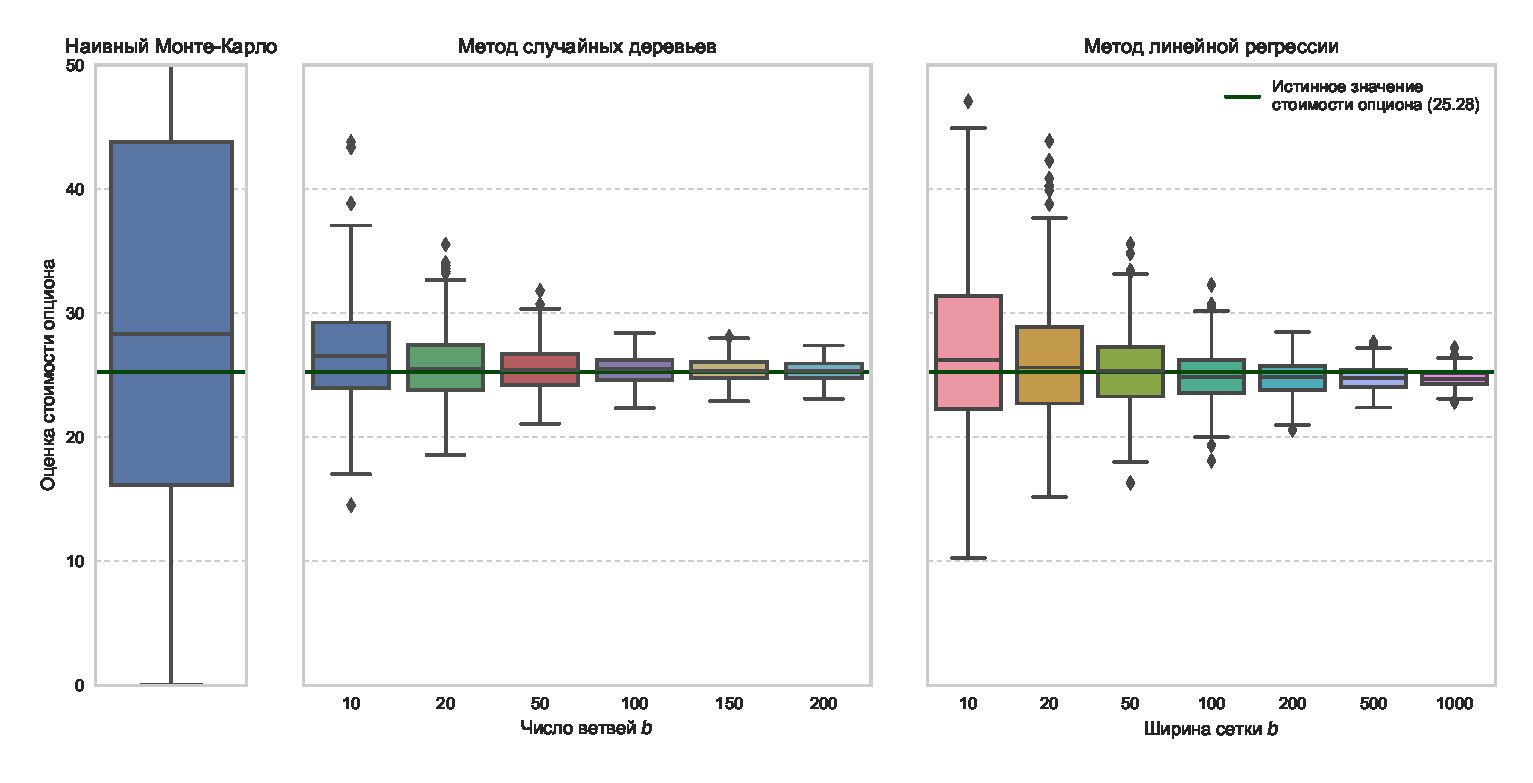
\includegraphics[width=\textwidth]{classical_methods.eps}
    \caption{Оценки стоимости опциона различными классическими методами}
    \footnotesize Оценки построены для примера \ref{example_3}. Из метода случайных деревьев взята оценка сверху. Вертикальная ось общая у всех трёх графиков.
    \label{fig:classical_methods}
\end{figure}

Здесь видно, что примерно одинаковый размер дисперсии (ориентироваться здесь имеет смысл на интерквартильный размах множества оценок, то есть высоту изображённого ящика) достигается в методе случайных деревьев при $b=100$ и в методе наименьших квадратов при $b=500$. Для случайного дерева для такого результата потребуется $\mathrm{dim} X_t \sum_{i=1}^{m-1 b^i} = 5 \cdot {1,010,100}$ обращений к генератору псевдослучайных чисел (обращения к генератору можно считать элементарной операцией, по количеству которых сравнивать время работы различных методов). В методе наименьших квадратов этот результат достигается за $\mathrm{dim} X_t \cdot (m-1)b = 5 \cdot 1500$ обращений, то есть оценку с той же дисперсией можно получить за гораздо меньшее время.

% section results:classical_approaches (end)

\section{Применение метода квази Монте-Карло к классическим методам} % (fold)
\label{sec:results:qmc_to_classical_methods}

В этом разделе обсуждаются результаты применения квази Монте-Карло к методам из предыдущей секции: методу случайных деревьев и методу наименьших квадратов. Были использованы две различные квазислучайные последовательности: квазислучайные числа Соболя \cite{NIEDERREITER198851} и квазислучайные числа Холтона \cite{Faure2009}.

Малые значения параметров алгоритмов используются специально для того, чтобы было возможным применить QMC и осуществить сравнение. В том числе по этой же причине сравнение приводится только для первых трёх примеров из списка выше: пример\,\ref{example_4} требует слишком большой размерности алгоритма для оценки. Несомненно, ограничения на размерность существующих последовательностей с низким дискрепансом серьёзно ограничивают область применения квазислучайных методов. Тем не менее, задачей работы было исследование самой возможности применения QMC для интегрирования сложных негладких функций (которой является стоимость Американского опциона), поэтому дискуссия о повышении размерности квазислучайной последовательности остаётся за рамками обсуждения.

Для каждой из последовательностей и каждого метода ниже приведено сравнение смещения и дисперсии (там, где её можно посчитать) оценок, полученных с использованием MC, QMC и RQMC. Подробное описание методики подсчёта дисперсии, стандартного отклонения и смещения приведено в секции \ref{ssub:qmc:randomization:variance_estimation}. Для каждой оценки было посчитано $N = 15,000$ реализаций, разделённых на $g = 600$ групп по $G = 25$ реализаций в каждой. 

\subsection{Последовательность Соболя} % (fold)
\label{sub:results:qmc_to_classical:sobol}

Квазислучайные числа Соболя показывают хорошие результаты интегрирования в умеренно высоких размерностях (см. \cite{sobol}). Примеры с использованием квазислучайных последовательностей Соболя различных размерностей посчитаны для размерностей, не превышающих 40. То есть, к примеру, если КРА (конструктивная размерность алгоритма) оценки по методу случайных деревьев превышает 40, то эта оценка не считается и не присутствует в таблицах результатов.

\subsubsection{Метод наименьших квадратов} % (fold)
\label{ssub:results:qmc_to_classical:sobol:lsm}

Результаты представлены на рис.\,\ref{fig:lsm_sobol} и в табл.\,\ref{tbl:lsm_sobol_ex1},\,\ref{tbl:lsm_sobol_ex2},\,\ref{tbl:lsm_sobol_ex3}.

\begin{figure}[p]
    \begin{center}
    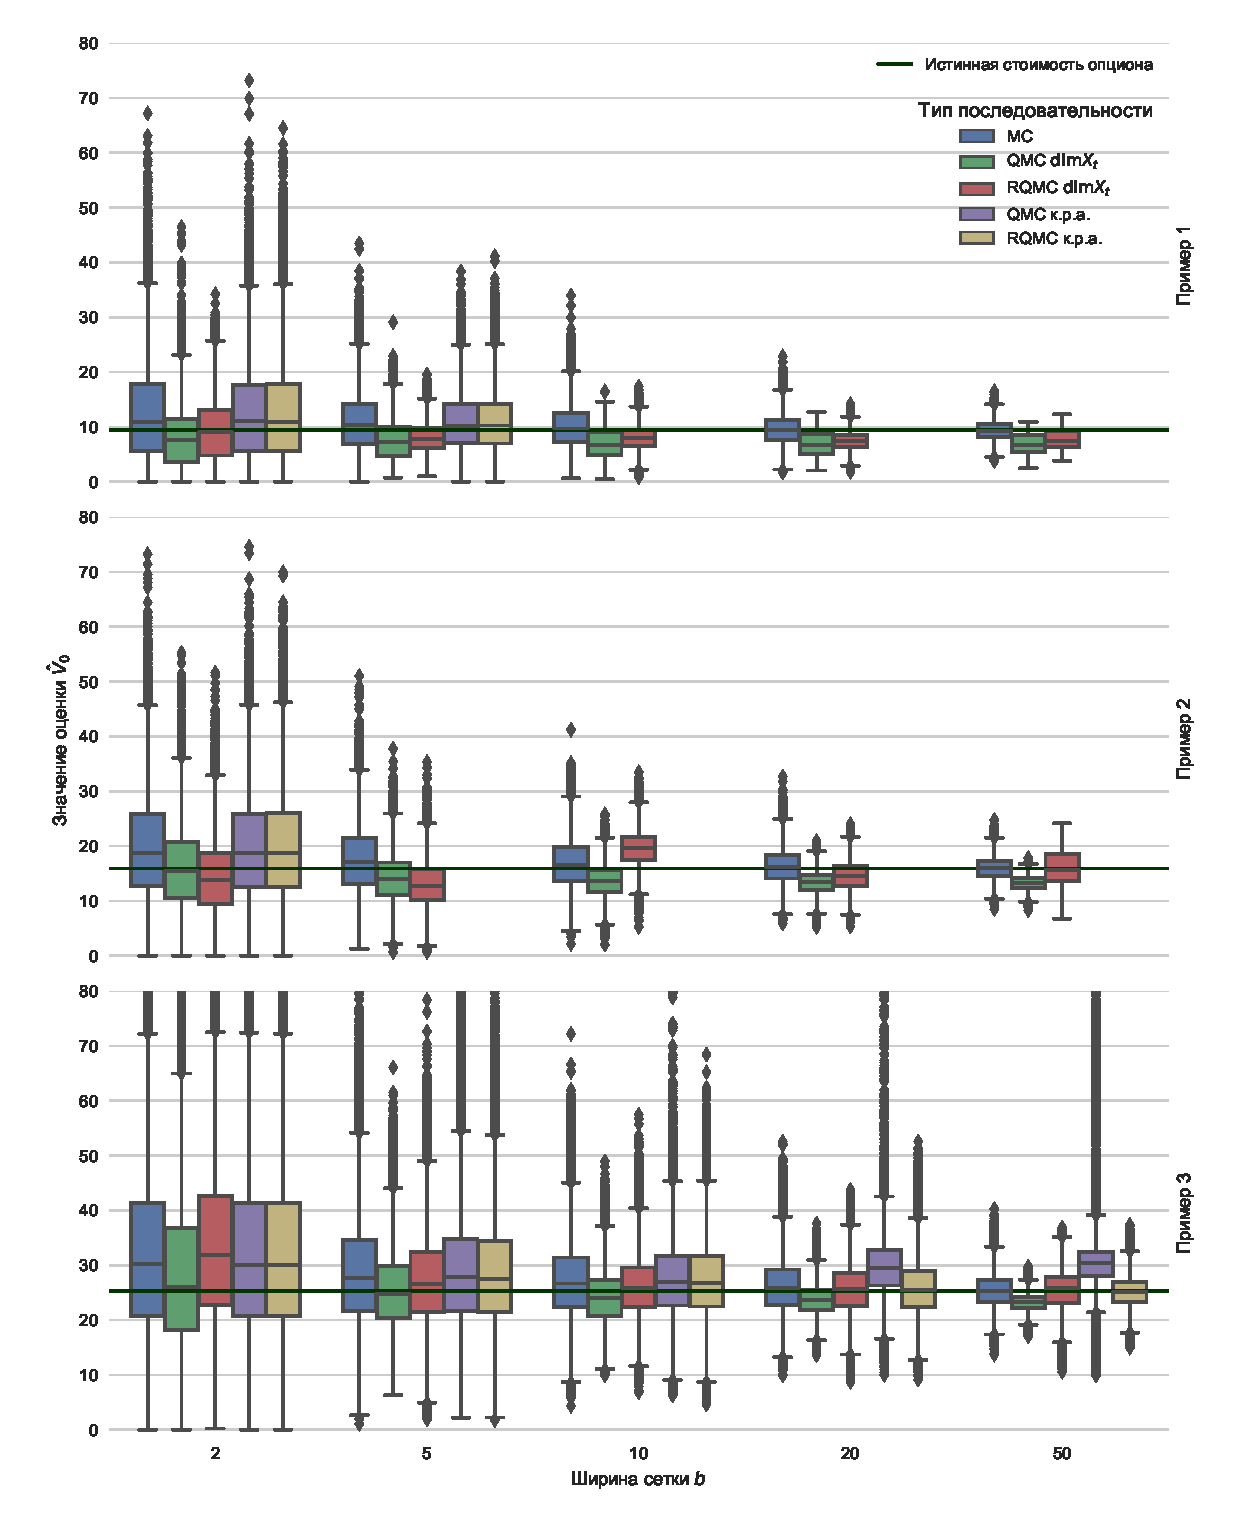
\includegraphics[width=0.9\textwidth]{lsm_sobol.eps}
    \end{center}
    \caption{Разброс оценок стоимости Американского опциона методом наименьших квадратов при использовании псевдослучайных последовательностей и квазислучайных последовательностей Соболя различных размерностей}
    \label{fig:lsm_sobol}

    \linespread{0.8}\footnotesize{На рисунке изображён именно разброс оценок, полученных при использовании различных отрезков квази- или псевдослучайной последовательности: подсчёт дисперсии и доверительных интервалов в случае QMC невозможен.}
\end{figure}

\begin{table}
    \renewcommand{\arraystretch}{0.6}
    \centering
    Оценки методом наименьших квадратов с псевдослучайной последовательностью (MC) и квазислучайной последовательностью Соболя (QMC)
    \caption{Пример 1}\label{tbl:lsm_sobol_ex1}
    \begin{tabular}{rrrrrrr}
        $b$&тип&$\mathrm{dim} X_t$&$\Vhat$&$\mathrm{sd}\Vhat$&$\mathrm{se}\Vhat$&$\mathrm{bias}\Vhat$\\[3pt]\hline\\[-8pt]
        2&MC&&12.562&1.856&3.700&3.201\\
        2&RQMC&2&9.516&1.112&1.123&0.155\\
        2&RQMC&12&12.535&1.139&3.372&3.174\\[3pt]
        5&MC&&10.992&1.045&1.937&1.631\\
        5&RQMC&2&7.938&0.606&1.546&-1.423\\
        5&RQMC&30&10.957&0.843&1.806&1.596\\[3pt]
        % 10&MC&&10.054&0.790&1.051&0.693\\
        % 10&RQMC&2&7.893&0.592&1.583&-1.468\\[3pt]
        % 20&MC&&9.562&0.501&0.540&0.201\\
        % 20&RQMC&2&7.403&0.697&2.078&-1.958\\[3pt]
        % 50&MC&&9.306&0.356&0.360&-0.055\\
        % 50&RQMC&2&7.673&1.480&2.245&-1.688\\[3pt]
    \end{tabular}

    \caption{Пример 2}\label{tbl:lsm_sobol_ex2}
    \begin{tabular}{rrrrrrr}
        $b$&тип&$\mathrm{dim} X_t$&$\Vhat$&$\mathrm{sd}\Vhat$&$\mathrm{se}\Vhat$&$\mathrm{bias}\Vhat$\\[3pt]\hline\\[-8pt]
        2&MC&&19.907&2.077&4.513&4.007\\
        2&RQMC&5&14.446&1.154&1.856&-1.454\\
        2&RQMC&30&19.851&1.528&4.236&3.951\\[3pt]
        5&MC&&17.557&1.270&2.088&1.657\\
        5&RQMC&5&13.058&1.205&3.087&-2.842\\[3pt]
        % 10&MC&&16.819&0.953&1.324&0.919\\
        % 10&RQMC&5&19.535&1.231&3.838&3.635\\[3pt]
        % 20&MC&&16.353&0.645&0.788&0.453\\
        % 20&RQMC&5&14.560&1.754&2.207&-1.340\\[3pt]
        % 50&MC&&15.983&0.435&0.443&0.083\\
        % 50&RQMC&5&15.958&2.682&2.682&0.058\\[3pt]
    \end{tabular}

    \caption{Пример 3}\label{tbl:lsm_sobol_ex3}
    \begin{tabular}{rrrrrrr}
        $b$&тип&$\mathrm{dim} X_t$&$\Vhat$&$\mathrm{sd}\Vhat$&$\mathrm{se}\Vhat$&$\mathrm{bias}\Vhat$\\[3pt]\hline\\[-8pt]
        2&MC&&32.438&3.421&7.934&7.158\\
        2&RQMC&30&32.285&7.987&10.623&7.005\\
        2&RQMC&5&35.431&1.825&10.314&10.151\\[3pt]
        5&MC&&28.570&1.990&3.845&3.290\\
        5&RQMC&5&25.258&2.010&2.010&-0.022\\[3pt]
        % 10&MC&&27.099&1.434&2.316&1.819\\
        % 10&RQMC&5&23.328&4.522&4.926&-1.952\\[3pt]
        % 20&MC&&26.110&0.941&1.255&0.830\\
        % 20&RQMC&5&26.001&0.943&1.187&0.721\\[3pt]
        % 50&MC&&25.418&0.605&0.621&0.138\\
        % 50&RQMC&5&24.545&2.455&2.563&-0.735\\[3pt]
    \end{tabular}

    \footnotesize{Расшифровку обозначений см.~в~\ref{eq:rqmc_variance_estimation}}
\end{table}

Результаты показывают, что использование квазислучайной последовательности Соболя размерности КРА снижает дисперсию оценки. Как и ожидалось, оценки с помощью квазислучайной последовательности размерности $\mathrm{dim} X$ не дают содержательных результатов: для некоторых случаев дисперсия меньше, чем в MC (пример 1, $b=2,5,10$; пример 2, $b=2$), для других --- меньше.

% subsubsection results:qmc_to_classical:sobol:lsm (end)

\subsubsection{Метод случайных деревьев} % (fold)
\label{ssub:results:qmc_to_classical:sobol:random_tree}

Результаты представлены на рис.\,\ref{fig:random_tree_sobol} и в табл.\,\ref{tbl:random_tree_sobol_ex1}.%,\,\ref{tbl:random_tree_sobol_ex2},\,\ref{tbl:random_tree_sobol_ex3}.

\begin{figure}[p]
    \begin{center}
    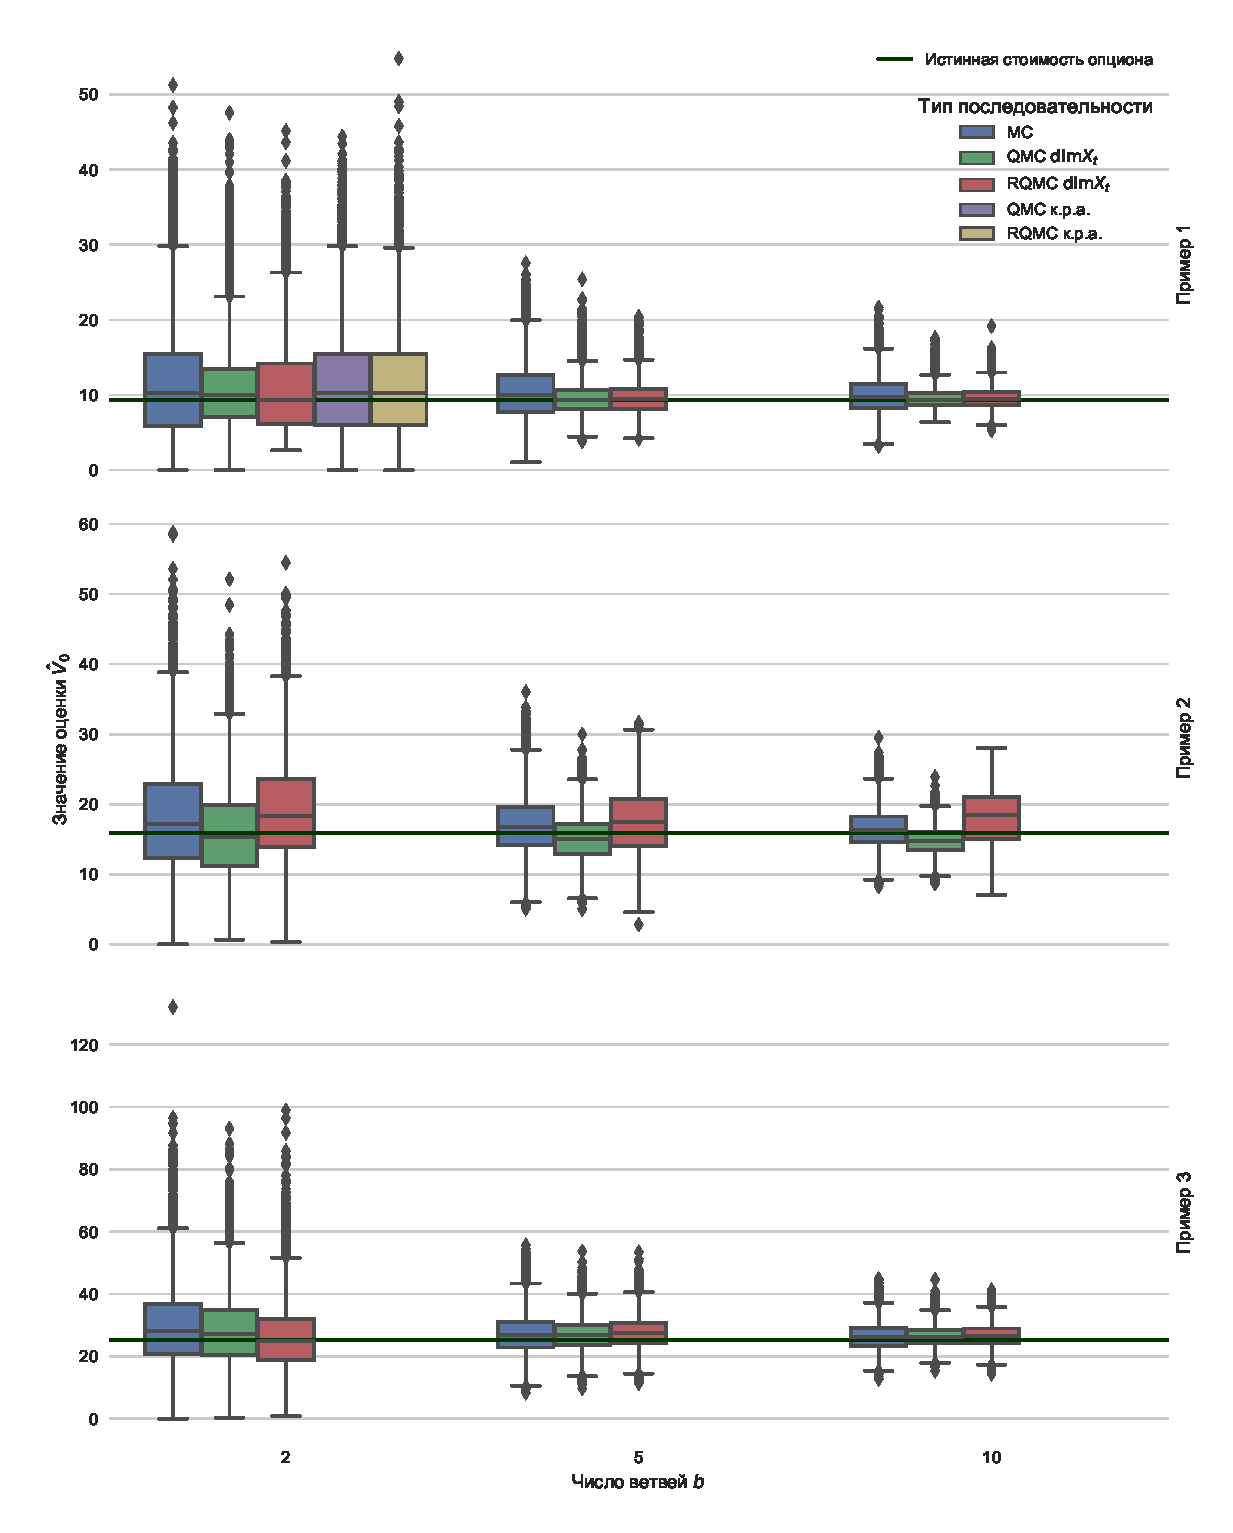
\includegraphics[width=0.9\textwidth]{random_tree_sobol.eps}\end{center}
    \caption{Разброс оценок стоимости Американского опциона методом случайных деревьев при использовании псевдослучайных последовательностей и квазислучайных последовательностей Соболя различных размерностей}
    \label{fig:random_tree_sobol}
    \linespread{0.8}\footnotesize{На рисунке изображён именно разброс оценок, полученных при использовании различных отрезков квази- или псевдослучайной последовательности: подсчёт дисперсии и доверительных интервалов в случае QMC невозможен.}
\end{figure}

\begin{table}
    \renewcommand{\arraystretch}{0.6}
    \centering
    Оценки методом случайных деревьев с псевдослучайной последовательностью (MC) и квазислучайной последовательностью Соболя (QMC)
    \caption{Пример 1}\label{tbl:random_tree_sobol_ex1}
    \begin{tabular}{rrrrrrr}
        $b$&тип&$\mathrm{dim} X_t$&$\Vhat$&$\mathrm{sd}\Vhat$&$\mathrm{se}\Vhat$&$\mathrm{bias}\Vhat$\\[3pt]\hline\\[-8pt]
        2&MC&&11.232&1.456&2.370&1.871\\
        2&RQMC&2&10.983&0.638&1.743&1.622\\
        2&RQMC&28&11.275&0.801&2.075&1.914\\[3pt]
        5&MC&&10.324&0.762&1.228&0.963\\
        5&RQMC&2&9.617&0.280&0.380&0.256\\[3pt]
  %       10&MC&&9.918&0.448&0.715&0.557\\
  %       10&RQMC&2&9.529&0.271&0.319&0.168\\[3pt]
  %       20&MC&&9.682&0.333&0.463&0.321\\
		% 20&RQMC&2&9.429&0.133&0.150&0.068\\[3pt]
    \end{tabular}

    % \caption{Пример 2}\label{tbl:random_tree_sobol_ex2}
    % \begin{tabular}{rrrrrrr}
    %     $b$&тип&$\mathrm{dim} X_t$&$\Vhat$&$\mathrm{sd}\Vhat$&$\mathrm{se}\Vhat$&$\mathrm{bias}\Vhat$\\[3pt]\hline\\[-8pt]
    %     2&MC&&17.934&1.570&2.570&2.034\\
    %     2&RQMC&5&19.065&2.004&3.746&3.165\\[3pt]
    %     5&MC&&16.990&0.807&1.356&1.090\\
    %     5&RQMC&5&17.414&3.428&3.748&1.514\\[3pt]
    %     10&MC&&16.499&0.536&0.803&0.599\\
    %     10&RQMC&5&18.016&3.273&3.897&2.116\\[3pt]
    % \end{tabular}

    % \caption{Пример 3}\label{tbl:random_tree_sobol_ex3}
    % \begin{tabular}{rrrrrrr}
    %     $b$&тип&$\mathrm{dim} X_t$&$\Vhat$&$\mathrm{sd}\Vhat$&$\mathrm{se}\Vhat$&$\mathrm{bias}\Vhat$\\[3pt]\hline\\[-8pt]
    %     2&MC&&29.502&2.432&4.873&4.222\\
    %     2&RQMC&5&26.231&2.573&2.743&0.951\\[3pt]
    %     5&MC&&27.207&1.228&2.285&1.927\\
    %     5&RQMC&5&27.666&2.017&3.124&2.386\\[3pt]
    %     10&MC&&26.353&0.811&1.346&1.073\\
    %     10&RQMC&5&26.673&1.720&2.213&1.393\\[3pt]
    % \end{tabular}

    \footnotesize{Расшифровку обозначений см.~в~\ref{eq:rqmc_variance_estimation}}
\end{table}

При использовании метода случайных деревьев только в одном случае КРА достаточно мала, чтобы строить оценку с использованием квазислучайной последовательности размерности, равной КРА. При этом остаётся неясным, насколько точными являются полученные оценки $\mathrm{sd}\Vhat$ и $\mathrm{se}\Vhat$ (возможно, если взять размер выборки $N$ чуть больше или чуть меньше, то отношение между $\mathrm{sd}\Vhat$ для MC и RQMC существенно изменится?). Одним из способов оценить поведение оценок является рис.\,\ref{fig:random_tree_sobol_variance}, на котором обсуждаемые оценки стандартного и среднеквадратичного отклонения изображены как функции от размера выборки. Он показывает, что оценки отклонений вполне статичны и преимущество RQMC в этом случае не является случайным эффектом малой выборки.

\begin{figure}[h!bt]
    \begin{center}
    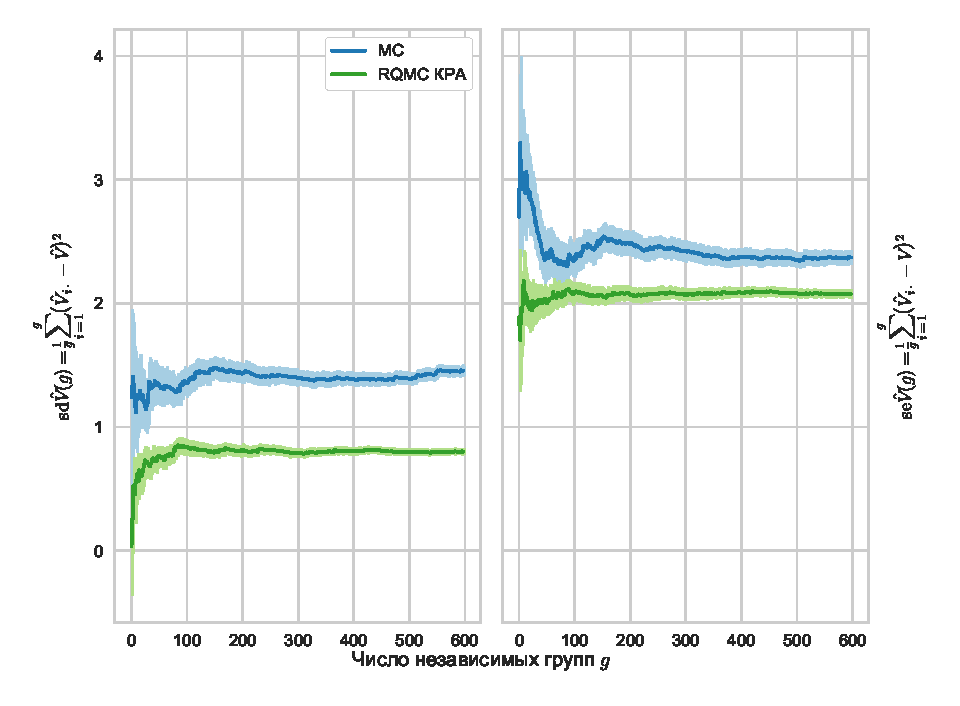
\includegraphics[width=0.9\textwidth]{random_tree_sobol_variance.eps}\end{center}
    \caption{Оценки $\mathrm{sd}\Vhat$ и $\mathrm{se}\Vhat$ в зависимости от размера выборки}
    \label{fig:random_tree_sobol_variance}
    \linespread{0.7}\footnotesize{
        Оценки стандартного и среднеквадратичного отклонения оценки стоимости Американского опциона из примера \ref{example_1} при использовании метода случайных деревьев с MC и RQMC Соболя размерности КРА. Количество коррелированных оценок в группе постоянно и равно $G=25$, при росте $g$ увеличивается размер выборки $N=g\cdot G$. Значения крайних правых точек графика указаны в табл.\,\ref{tbl:random_tree_sobol_ex1}. Значение оценки на выборке из первых $g$ групп указано более тёмной линией, более бледным обозначено стандартное отклонение этой оценки, посчитанное с помощью бутстрепа.}
\end{figure}

% subsubsection results:qmc_to_classical:sobol:random_tree (end)

% subsection results:qmc_to_classical:sobol (end)

\subsection{Последовательность Холтона} % (fold)
\label{sub:results:qmc_to_classical:halton}

Примеры с использованием квазислучайных последовательностей Холтона различных размерностей посчитаны для размерностей $< 40$. Стоит отметить, что в силу своей конструкции последовательности Холтона обычно не показывают хороших результатов при численном интегрировании в умеренно высоких размерностях (см., например, \cite{Faure2009}).

\subsubsection{Метод наименьших квадратов} % (fold)
\label{ssub:results:qmc_to_classical:halton:lsm}

Результаты представлены на рис.\,\ref{fig:lsm_halton} и в табл.\,\ref{tbl:lsm_halton_ex1},\,\ref{tbl:lsm_halton_ex2},\,\ref{tbl:lsm_halton_ex3}.

\begin{figure}[p]
    \begin{center}
    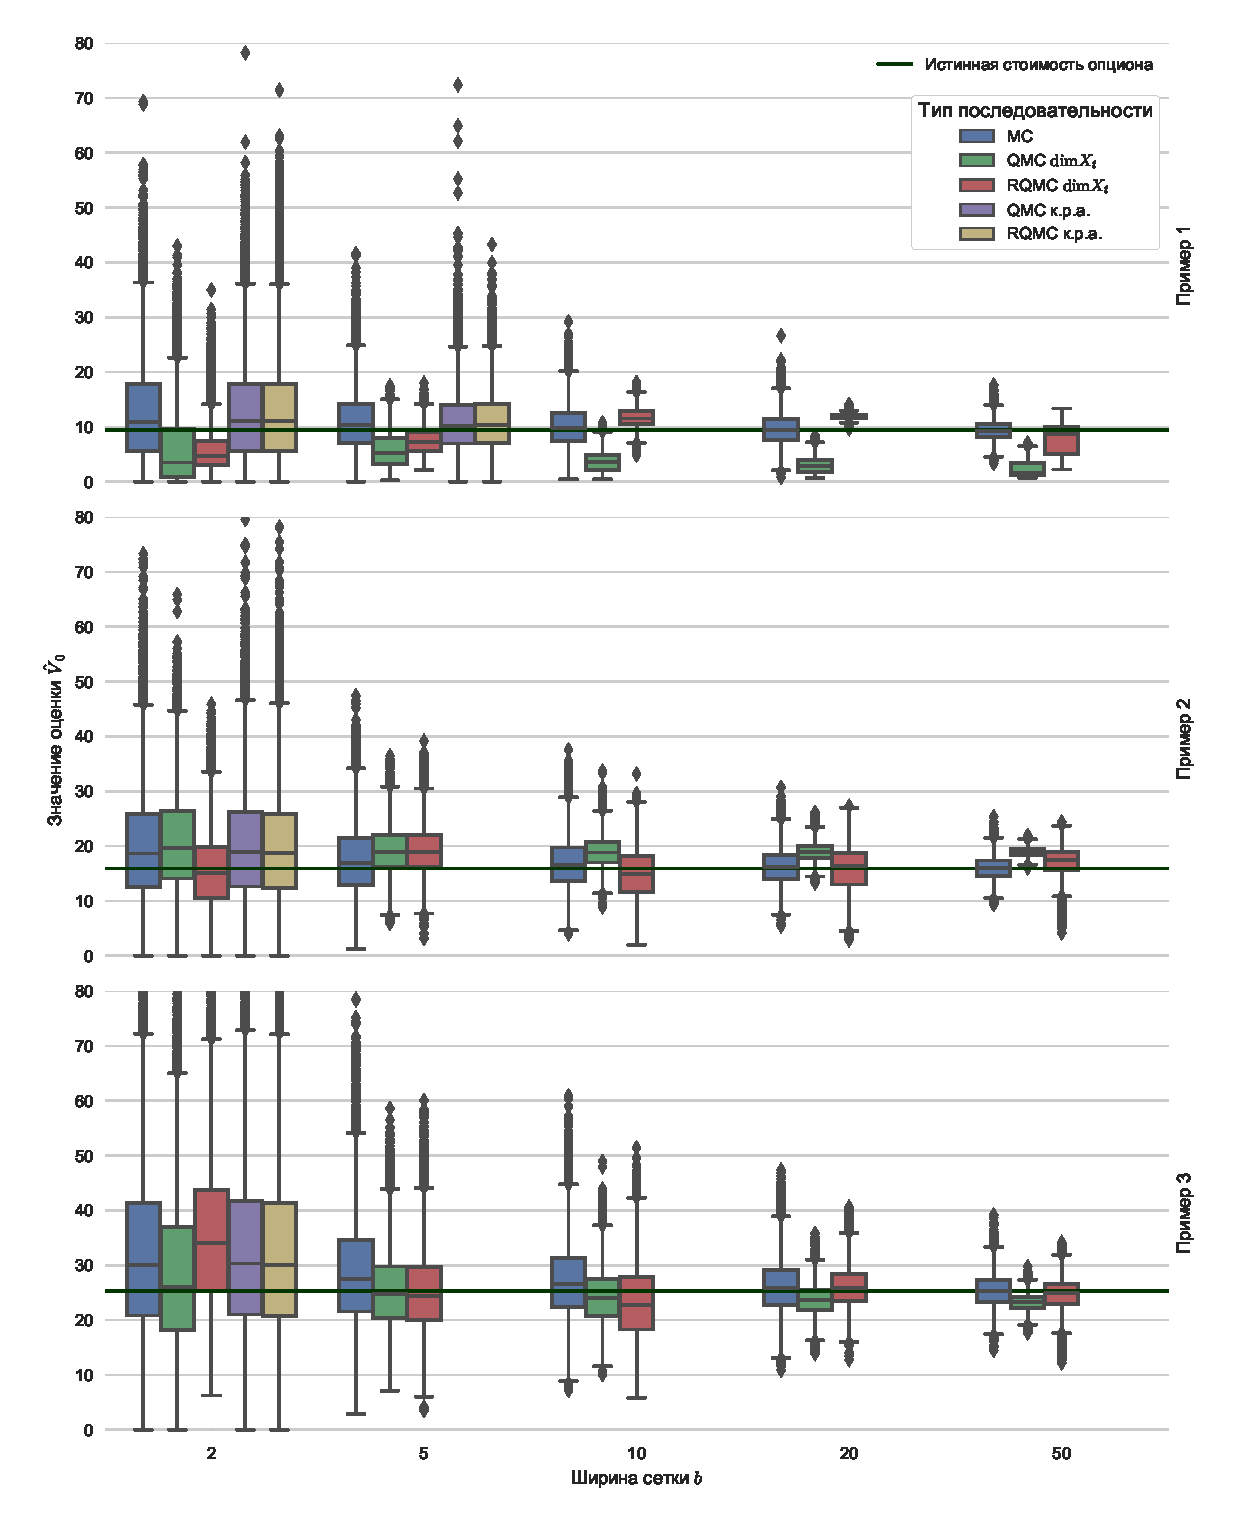
\includegraphics[width=0.9\textwidth]{lsm_halton.eps}\end{center}
    \caption{Разброс оценок стоимости Американского опциона методом наименьших квадратов при использовании псевдослучайных последовательностей и квазислучайных последовательностей Холтона различных размерностей}
    \label{fig:lsm_halton}
    \linespread{0.8}\footnotesize{На рисунке изображён именно разброс оценок, полученных при использовании различных отрезков квази- или псевдослучайной последовательности: подсчёт дисперсии и доверительных интервалов в случае QMC невозможен.}
\end{figure}

\begin{table}
    \renewcommand{\arraystretch}{0.6}
    \centering
    Оценки методом наименьших квадратов с псевдослучайной последовательностью и квазислучайной последовательностью Холтона
    \caption{Пример 1}\label{tbl:lsm_halton_ex1}
    \begin{tabular}{rrrrrrr}
        $b$&тип&$\mathrm{dim} X_t$&$\Vhat$&$\mathrm{sd}\Vhat$&$\mathrm{se}\Vhat$&$\mathrm{bias}\Vhat$\\[3pt]\hline\\[-8pt]
        2&MC&&12.535&1.818&3.658&3.174\\
        2&RQMC&12&12.540&2.339&3.947&3.179\\
        2&RQMC&2&6.119&0.543&3.287&-3.242\\[3pt]
        5&MC&&10.979&1.094&1.953&1.618\\
        5&RQMC&30&10.967&2.810&3.237&1.606\\
        5&RQMC&2&7.349&0.208&2.023&-2.012\\[3pt]
        10&MC&&10.120&0.736&1.058&0.759\\
        10&RQMC&2&11.696&0.117&2.338&2.335\\[3pt]
        % 20&MC&&9.639&0.549&0.615&0.278\\
        % 20&RQMC&2&11.867&0.064&2.507&2.506\\[3pt]
        % 50&MC&&9.292&0.348&0.355&-0.069\\
        % 50&RQMC&2&7.701&3.284&3.680&-1.660\\[3pt]
    \end{tabular}

    \caption{Пример 2}\label{tbl:lsm_halton_ex2}
    \begin{tabular}{rrrrrrr}
        $b$&тип&$\mathrm{dim} X_t$&$\Vhat$&$\mathrm{sd}\Vhat$&$\mathrm{se}\Vhat$&$\mathrm{bias}\Vhat$\\[3pt]\hline\\[-8pt]
        2&MC&&19.753&1.956&4.321&3.853\\
        2&RQMC&30&19.860&5.361&6.665&3.960\\
        2&RQMC&5&15.481&0.713&0.827&-0.419\\[3pt]
        5&MC&&17.478&1.243&2.009&1.578\\
        5&RQMC&5&19.220&0.622&3.377&3.320\\[3pt]
        % 10&MC&&16.822&0.903&1.291&0.922\\
        % 10&RQMC&5&15.008&3.358&3.474&-0.892\\[3pt]
        % 20&MC&&16.272&0.653&0.751&0.372\\
        % 20&RQMC&5&15.612&3.711&3.722&-0.288\\[3pt]
        % 50&MC&&16.011&0.429&0.443&0.111\\
        % 50&RQMC&5&16.647&3.263&3.348&0.747\\[3pt]
    \end{tabular}

    \caption{Пример 3}\label{tbl:lsm_halton_ex3}
    \begin{tabular}{rrrrrrr}
        $b$&тип&$\mathrm{dim} X_t$&$\Vhat$&$\mathrm{sd}\Vhat$&$\mathrm{se}\Vhat$&$\mathrm{bias}\Vhat$\\[3pt]\hline\\[-8pt]
        2&MC&&32.438&3.421&7.934&7.158\\
        2&RQMC&30&32.285&7.987&10.623&7.005\\
        2&RQMC&5&35.431&1.825&10.314&10.151\\[3pt]
        5&MC&&28.570&1.990&3.845&3.290\\
        5&RQMC&5&25.258&2.010&2.010&-0.022\\[3pt]
        % 10&MC&&27.099&1.434&2.316&1.819\\
        % 10&RQMC&5&23.328&4.522&4.926&-1.952\\[3pt]
        % 20&MC&&26.110&0.941&1.255&0.830\\
        % 20&RQMC&5&26.001&0.943&1.187&0.721\\[3pt]
        % 50&MC&&25.418&0.605&0.621&0.138\\
        % 50&RQMC&5&24.545&2.455&2.563&-0.735\\[3pt]
    \end{tabular}

    \footnotesize{Расшифровку обозначений см.~в~\ref{eq:rqmc_variance_estimation}}
\end{table}

Из таблиц \ref{tbl:lsm_halton_ex1},\,\ref{tbl:lsm_halton_ex2} видно, что на тех же примерах, где использование последовательность Соболя размерности, равной КРА, давало выигрыш в дисперсии, использование последовательности Холтона существенно увеличивает дисперсию. %Можно предположить, что эта разница объясняется тем, что в выборке слишком мало примеров. Но рис.\ref показывает, что во всех случаях оценки достаточно стабильны.

% subsubsection results:qmc_to_classical:halton:lsm (end)

\subsubsection{Метод случайных деревьев} % (fold)
\label{ssub:results:qmc_to_classical:halton:random_tree}

Результаты представлены на рис.\,\ref{fig:random_tree_halton} и в табл.\,\ref{tbl:random_tree_halton_ex1}.%,\,\ref{tbl:random_tree_halton_ex2},\,\ref{tbl:random_tree_halton_ex3}.

\begin{figure}[p]
    \begin{center}
    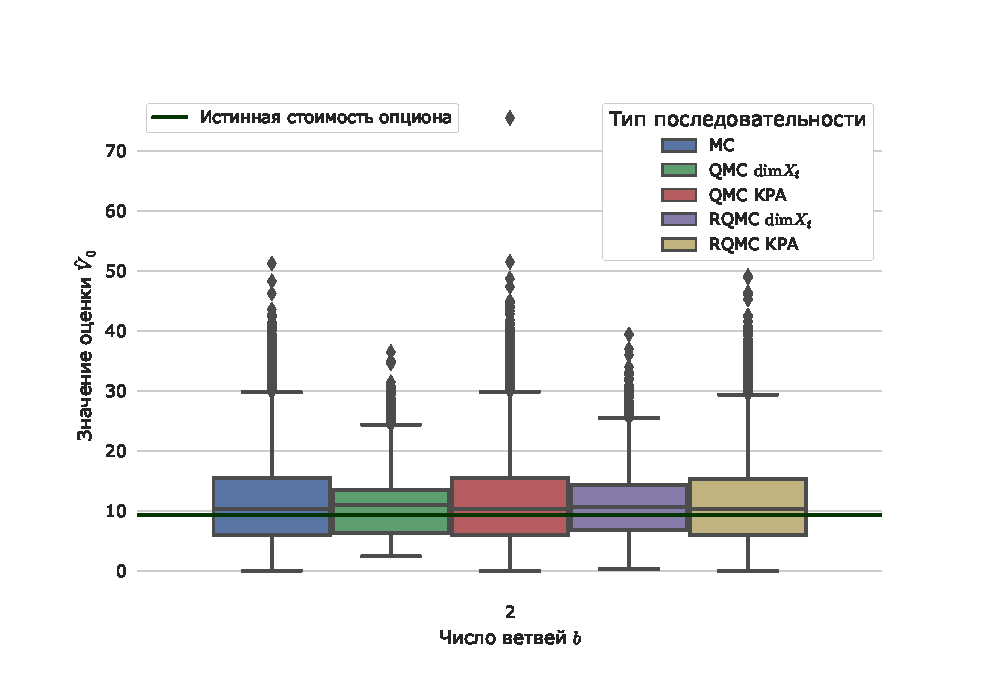
\includegraphics[width=0.9\textwidth]{random_tree_halton.eps}\end{center}
    \caption{Разброс оценок стоимости Американского опциона методом случайных деревьев при использовании псевдослучайных последовательностей (MC) и квазислучайных последовательностей Холтона (QMC) различных размерностей}
    \label{fig:random_tree_halton}
    \linespread{0.8}\footnotesize{На рисунке изображён именно разброс оценок, полученных при использовании различных отрезков квази- или псевдослучайной последовательности: подсчёт дисперсии и доверительных интервалов в случае QMC невозможен.}
\end{figure}

\begin{table}
    \renewcommand{\arraystretch}{0.6}
    \centering
    Оценки методом случайных деревьев с псевдослучайной последовательностью (MC) и квазислучайной последовательностью Холтона (QMC)
    \caption{Пример 1}\label{tbl:random_tree_halton_ex1}
    \begin{tabular}{rrrrrrr}
        $b$&тип&$d$&$\Vhat$&$\mathrm{sd}\Vhat$&$\mathrm{se}\Vhat$&$\mathrm{bias}\Vhat$\\[3pt]\hline\\[-8pt]
        2&MC&&11.232&1.456&2.370&1.871\\
        2&RQMC&2&11.014&0.429&1.708&1.653\\
        2&RQMC&28&11.273&1.969&2.745&1.912\\[3pt]
        5&MC&&10.324&0.762&1.228&0.963\\
        5&RQMC&2&9.879&0.217&0.562&0.518\\[3pt]
  %       10&MC&&9.918&0.448&0.715&0.557\\
  %       10&RQMC&2&9.559&0.465&0.505&0.198\\[3pt]
  %       20&MC&&9.682&0.333&0.463&0.321\\
  %       20&RQMC&2&9.423&0.110&0.126&0.062\\[3pt]
  %       50&MC&&9.490&0.190&0.230&0.129\\
		% 50&RQMC&2&9.376&0.041&0.044&0.015\\[3pt]
    \end{tabular}

    % \centering
    % \caption{Пример 2}\label{tbl:random_tree_halton_ex2}
    % \begin{tabular}{rrrrrrr}
    %     $b$&тип&$d$&$\Vhat$&$\mathrm{sd}\Vhat$&$\mathrm{se}\Vhat$&$\mathrm{bias}\Vhat$\\[3pt]\hline\\[-8pt]
    %     2&MC&&17.934&1.570&2.570&2.034\\
    %     2&RQMC&5&20.616&1.608&4.982&4.716\\[3pt]
    %     5&MC&&16.990&0.807&1.356&1.090\\
    %     5&RQMC&5&16.666&2.346&2.467&0.766\\[3pt]
    %     10&MC&&16.499&0.536&0.803&0.599\\
    %     10&RQMC&5&16.919&2.904&3.078&1.019\\[3pt]
    %     20&MC&&16.193&0.351&0.458&0.293\\
    %     20&RQMC&5&16.510&2.216&2.299&0.610\\[3pt]
    % \end{tabular}

    % \centering
    % \caption{Пример 3}\label{tbl:random_tree_halton_ex3}
    % \begin{tabular}{rrrrrrr}
    %     $b$&тип&$d$&$\Vhat$&$\mathrm{sd}\Vhat$&$\mathrm{se}\Vhat$&$\mathrm{bias}\Vhat$\\[3pt]\hline\\[-8pt]
    %     2&MC&&29.502&2.432&4.873&4.222\\
    %     2&RQMC&5&28.972&2.018&4.208&3.692\\[3pt]
    %     5&MC&&27.207&1.228&2.285&1.927\\
    %     5&RQMC&5&27.505&1.984&2.981&2.225\\[3pt]
    %     10&MC&&26.353&0.811&1.346&1.073\\
    %     10&RQMC&5&26.786&1.730&2.293&1.506\\[3pt]
    %     20&MC&&25.826&0.533&0.763&0.546\\
    %     20&RQMC&5&26.281&1.407&1.727&1.001\\[3pt]
    % \end{tabular}

    \footnotesize{Расшифровку обозначений см.~в~\ref{eq:rqmc_variance_estimation}}
\end{table}

Здесь, как и в случае с последовательностью Соболя (см. секцию\,\ref{ssub:results:qmc_to_classical:sobol:random_tree}), для КРА есть только одно наблюдение, поэтому стоит посмотреть на поведение отклонений в зависимости от размера выборки. Оно изображено на рис.\,\ref{fig:random_tree_halton_variance}. Судя по представленному на графике поведению, оценка стандартного отклонения для 600 наблюдений достаточно устойчива, и оснований считать, что QMC размерности КРА превосходит MC, нет.

% Про использование размерности, равной размерности актива, как и в случае с последовательностью Соболя, никаких выводов сделать нельзя: на примере \ref{example_1} (табл.\,\ref{tbl:random_tree_halton_ex1}) рандомизированный квази Монте-Карло демонстрирует стандартное отклонение намного меньшее стандартного отклонения классического Монте-Карло, тогда как в примерах \ref{example_2} и \ref{example_3} (табл.\,\ref{tbl:random_tree_halton_ex2} и \ref{tbl:random_tree_halton_ex3}) результаты гораздо хуже стандартного Монте-Карло. Также присутствует дополнительное смещение оценки.

\begin{figure}[h]
    \begin{center}
    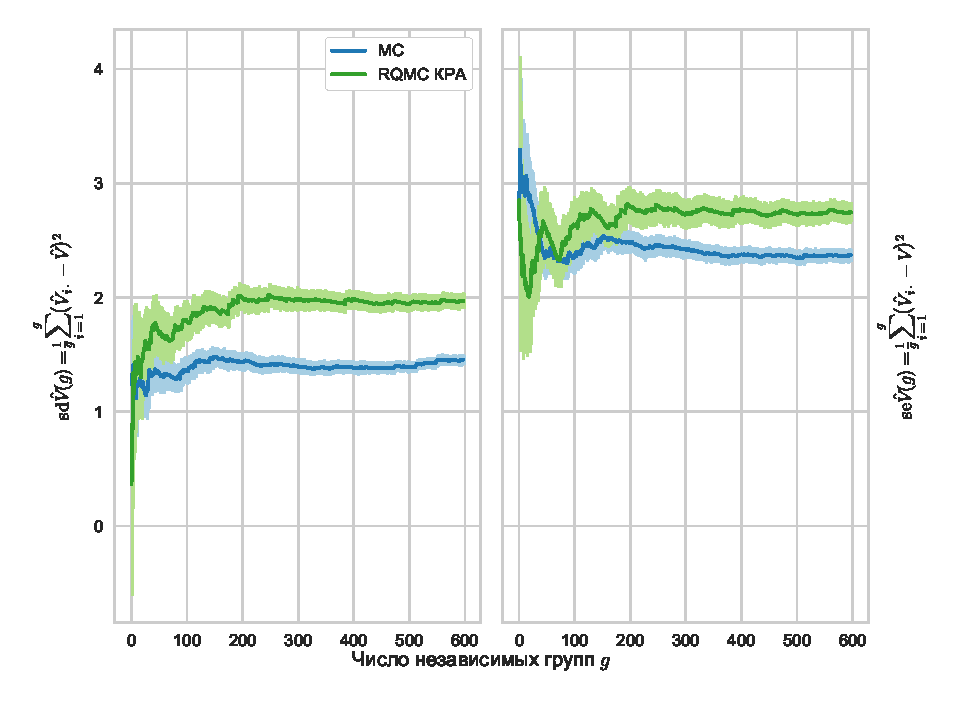
\includegraphics[width=0.9\textwidth]{random_tree_halton_variance.eps}\end{center}
    \caption{Оценки $\mathrm{sd}\Vhat$ и $\mathrm{se}\Vhat$ в зависимости от размера выборки}
    \label{fig:random_tree_halton_variance}
    \linespread{0.7}\footnotesize{
        Оценки стандартного и среднеквадратичного отклонения оценки стоимости Американского опциона из примера \ref{example_1} при использовании метода случайных деревьев с MC и c RQMC Холтона размерности, равной конструктивной размерности алгоритма. Количество коррелированных оценок в группе постоянно и равно $G=25$, при росте $g$ увеличивается размер выборки $N=g\cdot G$. Значения крайних правых точек графика указаны в табл.\,\ref{tbl:random_tree_sobol_ex1}. Значение оценки на выборке из первых $g$ групп указано более тёмной линией, более бледным обозначено стандартное отклонение этой оценки, посчитанное с помощью бутстрепа.}
\end{figure}

% subsubsection results:qmc_to_classical:halton:random_tree (end)

% subsection results:qmc_to_classical:halton (end)

Представленные в этом разделе результаты подтверждают, что последовательность Холтона плохо справляется с интегрированием в пространствах умеренно высокой размерности. Напротив, последовательность Соболя демонстрирует гораздо более хорошие результаты, чем классический Монте-Карло, даже в случае сложной негладкой функции.

% section results:qmc_to_classical_methods (end)

\section{Оценки по сглаженным случайным деревьям} % (fold)
\label{sec:results:pruned_trees}

Для сравнения алгоритмов требуется пример с известным ответом: Американский опцион с известными параметрами, для которого известна стоимость при условии возможности исполнения опциона в любой момент времени (т.е. при $m \to \infty$). Поэтому сравнение проводится для примера \ref{example_4}.

Оценка по сглаженным деревьям сравнивается с оценкой по методу наименьших квадратов. Параметры оценки по сглаженным деревьям ($b, h, n$) выбраны таким образом, чтобы доставлять наименьшую дисперсию при фиксированном $m$ и ограниченном сверху $n$. Параметр $b$ для метода наименьших квадратов выбирался таким образом, чтобы конструктивная размерность оценок совпадала. Сравнение дисперсий представлено на рис.\,\ref{fig:lsm_vs_pruned_variance}, и, согласно этим данным, дисперсия в методе сглаженных деревьев ниже.

\begin{figure}[h]
    \begin{center}
    \includegraphics[width=0.9\textwidth]{LSM_vs_pruned_variance.eps}\end{center}
    \caption{Дисперсия оценок по методу наименьших квадратов и методу сглаженных случайных деревьев}
    \label{fig:lsm_vs_pruned_variance}
\end{figure}

% section results:pruned_trees (end)

\section{Применение метода квази Монте-Карло к сглаженным случайным деревьям} % (fold)
\label{sec:results:qmc_to_pruned_trees}

Существует два наиболее очевидных варианта применения квази Монте-Карло к исследуемому методу:

\begin{enumerate}
	\item Использование QMC для генерирования более регулярной сетки на шаге выбора точек роста для новых деревьев: размерность QMC равна размерности базового актива, для генерации деревьев используется генератор псевдослучайных чисел (ГПСЧ).
	\item Использование QMC для генерации деревьев: размерность QMC равна $\mathrm{dim} X_t \cdot \sum_{i=1}^h b^i$, для выбора сетки используется ГПСЧ или другая QMC-последовательность (уже другой размерности).
\end{enumerate}

В таблицах далее эти варианты обозначаются суффиксами <<grid>> и <<tree>> соответственно. Сравнение оценок с использованием QMC с оценками с использованием MC приведено на рис.\,\ref{fig:pruned_tree_sobol} и в табл.\,\ref{tbl:pruned_tree_sobol}. Использовалась квазислучайная последовательность Соболя. Как видно из рисунка, использование QMC для генерации деревьев меньшую ошибку относительно истинного значения стоимости опциона. Это можно объяснить тем, что использование QMC для генерации сетки вершин обеспечивает более равномерную решётку, порождая более точные оценки линейной регрессии $\Vhat^{\mathrm{regr.}}_{p_l}$ и компенсируя тем самым один из источников смещения.

\begin{figure}[h]
    \begin{center}
    \includegraphics[width=0.9\textwidth]{pruned_tree_sobol.eps}\end{center}
    \caption{Разброс оценок стоимости Американского опциона методом сглаженных случайных деревьев при использовании псевдослучайных последовательностей (MC) и квазислучайных последовательностей Соболя (QMC) в различных частях алгоритма}
    \label{fig:pruned_tree_sobol}
    \linespread{0.8}\footnotesize{Вычисления представлены для примера \ref{example_4}. На рисунке изображён именно разброс оценок, полученных при использовании различных отрезков квази- или псевдослучайной последовательности: подсчёт дисперсии и доверительных интервалов в случае QMC невозможен.}
\end{figure}

Сведения из табл.\,\ref{tbl:pruned_tree_sobol} также демонстрируют, что использование рандомизированных квазислучайных методов не даёт большого выигрыша в дисперсии для оценки по сглаженным деревьям (по крайней мере, на исследуемом примере). При этом использование квазислучайных методов позволяет добиться разброса в значениях оценки по различным частям квазислучайной последовательности меньшего, чем в методе Монте-Карло (не указано в таблице).

\begin{table}
    \renewcommand{\arraystretch}{0.6}
    \centering
    \caption{Оценки методом сглаженных случайных деревьев при использовании псевдослучайных последовательностей (MC) и квазислучайных последовательностей Соболя (QMC) в различных частях алгоритма}\label{tbl:pruned_tree_sobol}
    \begin{tabular}{rrrrrrrrr}
    $b$&$h$&$m$&$n$&тип&$\Vhat$&$\mathrm{sd}\Vhat$&$\mathrm{se}\Vhat$&$\mathrm{bias}\Vhat$\\[3pt]\hline\\[-8pt]
    4&3&22&100&MC&12.952&0.371&3.336&3.315\\
    4&3&22&100&QMC grid&11.669&-&-&2.032\\
    4&3&22&100&QMC tree&2.373&-&-&-7.264\\
    4&3&22&100&RQMC grid&13.006&0.934&3.496&3.369\\
    4&3&22&100&RQMC tree&13.202&4.744&5.935&3.565\\[3pt]
    14&2&22&100&MC&13.321&0.224&3.691&3.684\\
    14&2&22&100&QMC grid&11.709&-&-&2.072\\
    14&2&22&100&QMC tree&2.532&-&-&-7.105\\
    14&2&22&100&RQMC grid&13.383&1.025&3.884&3.746\\
    14&2&22&100&RQMC tree&13.540&4.642&6.065&3.903\\[3pt]
    14&2&22&200&MC&13.379&0.208&3.748&3.742\\
    14&2&22&200&QMC grid&11.632&-&-&1.995\\
    14&2&22&200&QMC tree&2.458&-&-&-7.179\\
    14&2&22&200&RQMC grid&13.426&0.893&3.893&3.789\\
    14&2&22&200&RQMC tree&14.784&5.571&7.584&5.147\\[3pt]
    \end{tabular}
\end{table}
% section results:qmc_to_pruned_trees (end)
% chapter numerical_results (end)